%Jennifer Pan, August 2011

\documentclass[10pt,letter]{article}
	% basic article document class
	% use percent signs to make comments to yourself -- they will not show up.

\usepackage{amsmath}
\usepackage{amssymb}
	% packages that allow mathematical formatting
\DeclareMathOperator*{\argmax}{arg\,max}
\DeclareMathOperator*{\argmin}{arg\,min}
\usepackage{graphicx}
	% package that allows you to include graphics

\usepackage{setspace}
	% package that allows you to change spacing

\onehalfspacing
	% text become 1.5 spaced

\usepackage{fullpage}
	% package that specifies normal margins


\begin{document}
	% line of code telling latex that your document is beginning


\title{ECON500: Problem Set 2}

\author{Nicholas Wu}

\date{Fall 2020}
	% Note: when you omit this command, the current dateis automatically included

\maketitle
	% tells latex to follow your header (e.g., title, author) commands.


\section*{Part 1}

\paragraph{(1.1)}
Homogeneity follows from the nature of the budget constraint; given that the maximization problem is given by
\[ \max u(x) \]
\[ p \cdot x \le w \]
But the constraint $p \cdot x \le w$ holds if and only if $\alpha p \cdot x \le \alpha w$. Hence the maximizer $x^*(p,w) = x^*(\alpha p, \alpha w)$, since the maximization problems are equivalent. So the demand is homogeneous of degree 0.

For the next two parts, we suppose the utility is weakly monotonic.
To show Walras' law, suppose $x^*(p,w)$ is a maximizer for the utility maximization problem, but suppose $p\cdot x^* < w$. Let $p\cdot x^* = w^*$. Then since $w^* < w$, $w/w^* > 1$. So $p \cdot (w/w^*)x^* = w$. Further, $(w/w^*) x^* \ge x^*$ in all dimensions since $w/w^* > 1$. By monotonicity, this implies $u((w/w^*) x^*) \ge u(x^*)$, a violation of our assumption that $x^*$ maximized $u$. Hence Walras' law holds.

Now, we show WARP holds. Suppose $x(p,w)$ is chosen at $(p,w)$, and $x(p,w)$ is affordable at $(p',w')$: that is,
\[ p' x(p,w) \le w' \]
Then by utility maximization, we must have $u(x(p',w')) \ge u(x(p,w))$. But $x(p,w)$ maximized utility at $(p,w)$, thus, we cannot have $x(p',w')$ in the feasible set for $(p,w)$. This implies $px(p',w') > w$, and hence WARP holds.

Finally, we show that if $u$ is not monotonic, Walras' law and WARP need not hold. Consider utility $u(x) = -(x+ y - 1)^2$. Then it is possible that at $(p=(1,1), w=2)$, the bundle $x = (1,0)$ is chosen, even though $x\cdot p = 1 < 2$. Further, at prices $(p'=(1, 2), w'=2)$, it is possible that $x' = (0,1)$ is chosen (it is a utility maximizer), but we know that both $x=(0,1)$ and $x'=(1,0)$ are feasible for $(p=(1,1), w=2)$ as well as $(p'=(1,2), w'=2)$. Hence in this example, both WARP and Walras' law need not hold.


\paragraph{(1.2)}
Clearly, WARP implies WARP for compensated price changes. It suffices to show that if WARP fails, there exists a compensated price change for which WARP fails (this implies that WARP holds iff it holds for compensated price changes). Suppose WARP fails, and for some $x(p,w) \neq x(p',w')$,
\[ p' x(p,w) \le w'  \]
but
\[ p x(p',w') \le w \]
If $p' x(p,w) = w'$, then $(p',w')$ is a compensated price change to $(p,w)$, and we have a violation of WARP for a compensated price change. Likewise, if $p x(p',w') = w$, then $(p,w)$  is a compensated price change to $(p',w')$. If neither, then we have the strict inequalities:
\[ p'x(p,w) < w' \]
and
\[ px(p',w') < w \]
This implies
\[ p'x(p,w) - w' < 0 < w - px(p',w') \]
By Walras' law,
\[ p'x(p,w) - p'x(p',w') < 0 < px(p,w) - px(p',w') \]
\[ p'(x(p,w) - x(p',w')) < 0 < p(x(p,w) - x(p',w'))\]
By the IVT, we have that $\exists p''$ between $p'$ and $p$ such that
\[ p''(x(p,w) - x(p',w')) = 0 \]
Then define $w'' = p''x(p,w) = p''x(p',w')$. We now want to think of $p'', w''$ as a compensated price change to $(p,w)$ or $(p', w')$. Hence, WARP is violated if $x(p'',w'')$ is affordable at either $(p,w)$ or $(p', w')$.
However, note that since $p''$ is a convex combination of $p', p$, we get that for some $\lambda$,
\[ p''x(p'',w'') = p''x(p, w) = \lambda p x(p,w) + (1-\lambda) p'x(p,w) \]
\[ = \lambda w + (1-\lambda ) p'x(p,w) \]
but by our supposition, $p'x(p,w) < w'$, so
\[ p''x(p'',w'') < \lambda w + (1-\lambda) w' \]
\[ \lambda p x''(p,w) + (1-\lambda) p'x''(p,w)< \lambda w + (1-\lambda) w' \]
Hence we must have either $px(p'',w'') \le w$ or $p'x''(p,w) \le w'$ in order for this inequality to hold. But this implies that $x(p'', w'')$ is affordable at $(p,w)$ or $(p',w')$, and both are compensated price changes to $(p'', w'')$, so we have a violation. Hence, WARP holds iff it holds for compensated price changes.

Now, we show WARP holds iff WARP holds for price vectors that sum to 1. Once again, it is trivial that WARP implies WARP holds for price vectors with L1 norm 1. Hence, we just need to show that if WARP fails, it must fail for some price vectors with L1 norm equal to 1. Suppose WARP fails, that is there exists $(p,w), (p',w')$ and $x(p,w) \neq x(p',w')$, and
\[ p x(p', w') \le w \]
\[ p' x(p, w) \le w'\]
Let $\sum_i p_i =  s$, $\sum_i p'_i =  s'$. Consider $(p/s, w/s)$ and $(p'/s', w'/s')$. Then by homogeneity,
\[ \frac{p}{s} x(p'/s', w'/s') = \frac{p}{s} x(p', w') \le \frac{w}{s} \]
\[ \frac{p'}{s} x(p/s, w/s) = \frac{p'}{s} x(p, w) \le \frac{w'}{s} \]
But this is a violation of WARP on $(p/s, w/s)$ and $(p'/s', w'/s')$. We can easily confirm that the L1 norms of $p/s$ and $p'/s'$ are both 1, and hence a violation of WARP implies a violation of WARP on price vectors with L1 norm equal to 1.

More generally, we can show that for a strictly increasing, continuous $f$, with $f(0) = 0$ and $\lim_{a \to \infty} f(ap) > 1$ for all $p \neq 0$, we can show that WARP holds iff WARP holds for the price vectors such that $f(p) = 1$. Once again, the forward direction is obvious; clearly WARP implies WARP for $p$ such that $f(p) = 1$. In the reverse direction, suppose WARP fails. Then $\exists (p,w), (p',w')$, such that $x(p,w) \neq x(p',w')$. If we suppose that $
\lim_{\alpha \to \infty} f(\alpha p) > 1$, then since $f(0p) = 0$, it follows by the intermediate value theorem and the continuity of $f$ that some $a$ exists such that $f(ap) = 1$. Likewise, some $a'$ exists such that $f(a'p') = 1$. Then if we consider $(ap, aw)$ and $(a'p', a'w')$, we have from homogeneity that
\[ ap x(a'p', a'w') =  ap x(p',w') \le a w \]
and
\[ a'p' x(ap, aw) = a'p' x(p,w) \le a'w' \]
Hence, we have a violation of WARP between $(ap, aw)$ and $(a'p', a'w')$. By definition $f(ap) = f(a'p') = 1$, and hence we are done.

\paragraph{(1.3)}
We take the general form:
\[ u(x) = \left( \sum_{i=1}^N \alpha_i x_i^\rho \right)^{1/\rho} \]
The first order conditions are given by:
\[ \frac{\partial u}{\partial x_k} = \alpha_k\left( \sum_{i=1}^N \alpha_i x_i^\rho \right)^{(1/\rho) - 1} x_k^{\rho - 1} = \lambda p_k \]
Equivalently,
\[ \alpha_k\left( \sum_{i=1}^N \alpha_i x_i^\rho \right)^{(1/\rho) - 1} x_k^{\rho} = \lambda p_k x_k \]
Summing over all $k$, we get
\[ \left( \sum_{i=1}^N \alpha_i x_i^\rho \right)^{(1/\rho) - 1} \sum_{k=1}^N \alpha_k x_k^{\rho} = \lambda w \]
\[ \left( \sum_{i=1}^N \alpha_i x_i^\rho \right)^{(1/\rho)} = \lambda w \]
\[ \lambda = \frac{1}{w}\left( \sum_{i=1}^N \alpha_i x_i^\rho \right)^{(1/\rho)} \]
Plugging in our Lagrange multiplier to the FOC, we get
\[ \alpha_k\left( \sum_{i=1}^N \alpha_i x_i^\rho \right)^{(1/\rho) - 1} x_k^{\rho - 1} = \frac{p_k}{w}\left( \sum_{i=1}^N \alpha_i x_i^\rho \right)^{(1/\rho)} \]
\[ \alpha_k x_k^{\rho - 1}\left( \sum_{i=1}^N \alpha_i x_i^\rho \right)^{- 1}  = \frac{p_k}{w} \]
\[ \alpha_k x_k^{\rho - 1}  = \frac{p_k}{w}\left( \sum_{i=1}^N \alpha_i x_i^\rho \right) \]
\[ x_k^{\rho - 1}  = \frac{p_k}{\alpha_k}\left( \frac{1}{w}\sum_{i=1}^N \alpha_i x_i^\rho \right) \]
\[ x_k = \left(\frac{p_k}{\alpha_k}\right)^{\frac{1}{\rho-1}}\left( \frac{1}{w}\sum_{i=1}^N \alpha_i x_i^\rho \right)^{\frac{1}{\rho-1}} \]
Note the sum term is the same for all $k$. Working to eliminate this, we get
\[ x_k^\rho = \left(\frac{p_k}{\alpha_k}\right)^{\frac{\rho}{\rho-1}}\left( \frac{1}{w}\sum_{i=1}^N \alpha_i x_i^\rho \right)^{\frac{\rho}{\rho-1}} \]
\[ \alpha_k x_k^\rho = \frac{p_k^{\frac{\rho}{\rho-1}}}{\alpha_k^{\frac{1}{\rho-1} }}\left( \frac{1}{w}\sum_{i=1}^N \alpha_i x_i^\rho \right)^{\frac{\rho}{\rho-1}} \]
\[ \sum \alpha_k x_k^\rho = \left(\sum \frac{p_k^{\frac{\rho}{\rho-1}}}{\alpha_k^{\frac{1}{\rho-1} }} \right)\left( \frac{1}{w}\sum_{i=1}^N \alpha_i x_i^\rho \right)^{\frac{\rho}{\rho-1}} \]
\[ \sum_{k=1}^N \alpha_k x_k^\rho =  \left(\sum_{k=1}^N \left(\frac{p_k^\rho}{\alpha_k w^\rho}\right)^{\frac{1}{\rho-1}} \right)\left(\sum_{i=1}^N \alpha_i x_i^\rho \right)^{\frac{\rho}{\rho-1}} \]
\[ \left( \sum_{k=1}^N \alpha_k x_k^\rho \right)^{\frac{1}{\rho-1}} =  \left(\sum_{k=1}^N \left(\frac{p_k^\rho}{\alpha_k w^\rho}\right)^{\frac{1}{\rho-1}} \right)^{-1} \]
Plugging back in, we get
\[ x_k = \left(\frac{p_k}{\alpha_k}\right)^{\frac{1}{\rho-1}}\left( \frac{1}{w}\sum_{i=1}^N \alpha_i x_i^\rho \right)^{\frac{1}{\rho-1}} \]
\[ x_k = \left(\frac{p_k}{\alpha_k w}\right)^{\frac{1}{\rho-1}}\left(\sum_{k=1}^N \left(\frac{p_k^\rho}{\alpha_k w^\rho}\right)^{\frac{1}{\rho-1}} \right)^{-1} \]
\[ x_k = w \left(\frac{p_k}{\alpha_k}\right)^{\frac{1}{\rho-1}}\left(\sum_{k=1}^N \left(\frac{p_k^\rho}{\alpha_k }\right)^{\frac{1}{\rho-1}} \right)^{-1} \]
\[ x_k = w \left(\frac{\alpha_k}{p_k}\right)^{\frac{1}{1-\rho}}\left(\sum_{i=1}^N \left(\alpha_i p_i^{-\rho }\right)^{\frac{1}{1-\rho}} \right)^{-1} \]
\paragraph{(1.4)}
We first compute the partial derivative:
\[ \frac{\partial x_l}{\partial p_k} =  \frac{\rho}{1-\rho}w \left(\frac{\alpha_l}{p_l}\right)^{\frac{1}{1-\rho}}\left(\sum_{i=1}^N \left(\frac{\alpha_i}{p_i^\rho }\right)^{\frac{1}{1-\rho}} \right)^{-2} \left(\alpha_k^{\frac{1}{1-\rho}}p_k^{\frac{-\rho}{1-\rho} - 1} \right) \]
\[  =  \frac{\rho}{1-\rho}w \left(\frac{\alpha_l\alpha_k}{p_lp_k}\right)^{\frac{1}{1-\rho}}\left(\sum_{i=1}^N \left(\frac{\alpha_i}{p_i^\rho }\right)^{\frac{1}{1-\rho}} \right)^{-2}  \]
For an off-diagonal entry:
\[ S_{lk} = \frac{\partial x_l}{\partial p_k} + \frac{\partial x_l}{\partial w} x_k \]
\[ =  \frac{\rho}{1-\rho}w \left(\frac{\alpha_l\alpha_k}{p_lp_k}\right)^{\frac{1}{1-\rho}}\left(\sum_{i=1}^N \left(\frac{\alpha_i}{p_i^\rho }\right)^{\frac{1}{1-\rho}} \right)^{-2} + w \left(\frac{\alpha_k\alpha_l}{p_kp_l}\right)^{\frac{1}{1-\rho}}\left(\sum_{i=1}^N \left(\alpha_i p_i^{-\rho }\right)^{\frac{1}{1-\rho}} \right)^{-2} \]
\[ =  \frac{w}{1-\rho}\left(\frac{\alpha_l\alpha_k}{p_lp_k}  \right)^{\frac{1}{1-\rho}}\left(\sum_{i=1}^N \left(\frac{\alpha_i}{p_i^\rho }\right)^{\frac{1}{1-\rho}} \right)^{-2}  \]
For the symmetric case, we first compute:
\[ \frac{\partial x_k}{\partial p_k} =  w\left(  -\frac{1}{1-\rho}\left(\alpha_k p_k^{\rho-2}\right)^{\frac{1}{1-\rho}}\left(\sum_{i=1}^N \left(\alpha_i p_i^{-\rho }\right)^{\frac{1}{1-\rho}} \right)^{-1}  + \frac{\rho}{1-\rho} \left(\frac{\alpha_k^2}{p_k^2}\right)^{\frac{1}{1-\rho}}\left(\sum_{i=1}^N \left(\alpha_i p_i^{-\rho }\right)^{\frac{1}{1-\rho}} \right)^{-2} \right) \]
The Slutsky matrix entry on the diagonal is then
\[ S_{kk} = w\left(  -\frac{1}{1-\rho}\left(\alpha_k p_k^{\rho-2}\right)^{\frac{1}{1-\rho}}\left(\sum_{i=1}^N \left(\alpha_i p_i^{-\rho }\right)^{\frac{1}{1-\rho}} \right)^{-1}  + \frac{1}{1-\rho} \left(\frac{\alpha_k^2}{p_k^2}\right)^{\frac{1}{1-\rho}}\left(\sum_{i=1}^N \left(\alpha_i p_i^{-\rho }\right)^{\frac{1}{1-\rho}} \right)^{-2}  \right) \]
\[  = -\frac{w}{1-\rho}\left( \left(\alpha_k p_k^{\rho-2}\right)^{\frac{1}{1-\rho}}\left(\sum_{i=1}^N \left(\alpha_i p_i^{-\rho }\right)^{\frac{1}{1-\rho}} \right)^{-1}  - \left(\frac{\alpha_k^2}{p_k^2}\right)^{\frac{1}{1-\rho}}\left(\sum_{i=1}^N \left(\alpha_i p_i^{-\rho }\right)^{\frac{1}{1-\rho}} \right)^{-2}  \right) \]
\[  = -\frac{w}{1-\rho}\left(\frac{\alpha_k}{p_k^2} \right)^{\frac{1}{1-\rho}}\left( p_k^{\frac{\rho}{1-\rho}}\left(\sum_{i=1}^N \left(\alpha_i p_i^{-\rho }\right)^{\frac{1}{1-\rho}} \right)  - \alpha_k^{\frac{1}{1-\rho}}  \right)\left(\sum_{i=1}^N \left(\alpha_i p_i^{-\rho }\right)^{\frac{1}{1-\rho}} \right)^{-2} \]
\[  = -\frac{w}{1-\rho}\left(\frac{\alpha_k}{p_k^2} \right)^{\frac{1}{1-\rho}}\left( \left(\sum_{i=1}^N \left( \frac{\alpha_i p_k^\rho}{p_i^\rho} \right)^{\frac{1}{1-\rho}} \right)  - \alpha_k^{\frac{1}{1-\rho}}  \right)\left(\sum_{i=1}^N \left(\frac{\alpha_i}{p_i^\rho }\right)^{\frac{1}{1-\rho}} \right)^{-2} \]
\paragraph{(1.5)}
We let
\[ w(p) = p \cdot x(\tilde{p}, \tilde{w}) \]
\[ = \sum_{k=1}^N p_k \tilde{w} \left(\frac{\alpha_k}{\tilde{p_k}}\right)^{\frac{1}{1-\rho}}\left(\sum_{i=1}^N \left(\alpha_i \tilde{p_i}^{-\rho }\right)^{\frac{1}{1-\rho}} \right)^{-1} \]
We now consider
\[ x(p, w(p))_k = w(p) \left(\frac{\alpha_k}{p_k}\right)^{\frac{1}{1-\rho}}\left(\sum_{i=1}^N \left(\alpha_i p_i^{-\rho }\right)^{\frac{1}{1-\rho}} \right)^{-1} \]
Then
\[ \frac{\partial x(p, w(p))_l}{\partial p_k} = \frac{\partial w(p)}{\partial p_k} \left(\frac{\alpha_l}{p_l}\right)^{\frac{1}{1-\rho}}\left(\sum_{i=1}^N \left(\alpha_i p_i^{-\rho }\right)^{\frac{1}{1-\rho}} \right)^{-1} + \frac{\rho}{1-\rho}w(p)\left(\frac{\alpha_l\alpha_k}{p_lp_k}\right)^{\frac{1}{1-\rho}}\left(\sum_{i=1}^N \left(\alpha_i p_i^{-\rho }\right)^{\frac{1}{1-\rho}} \right)^{-2} \]
\[ = w \left(\frac{\alpha_l\alpha_k}{p_lp_k}\right)^{\frac{1}{1-\rho}}\left(\sum_{i=1}^N \left(\alpha_i p_i^{-\rho }\right)^{\frac{1}{1-\rho}} \right)^{-2} + \frac{\rho}{1-\rho}w(p)\left(\frac{\alpha_l\alpha_k}{p_lp_k}\right)^{\frac{1}{1-\rho}}\left(\sum_{i=1}^N \left(\alpha_i p_i^{-\rho }\right)^{\frac{1}{1-\rho}} \right)^{-2} \]
\[ = \frac{w}{1-\rho}\left(\frac{\alpha_l\alpha_k}{p_lp_k}\right)^{\frac{1}{1-\rho}}\left(\sum_{i=1}^N \left(\alpha_i p_i^{-\rho }\right)^{\frac{1}{1-\rho}} \right)^{-2} \]
\[ = S_{lk} \]
In the symmetric case,
\[ \frac{\partial x(p, w(p))_k}{\partial p_k} = \frac{\partial w(p)}{\partial p_k} \left(\frac{\alpha_k}{p_k}\right)^{\frac{1}{1-\rho}}\left(\sum_{i=1}^N \left(\alpha_i p_i^{-\rho }\right)^{\frac{1}{1-\rho}} \right)^{-1} - \frac{1}{1-\rho}w(p)\left(\frac{\alpha_k}{p_k^{2-\rho}}\right)^{\frac{1}{1-\rho}}\left(\sum_{i=1}^N \left(\alpha_i p_i^{-\rho }\right)^{\frac{1}{1-\rho}} \right)^{-1}\]\[ + \frac{\rho}{1-\rho}w(p)\left(\frac{\alpha_k^2}{p_k^2}\right)^{\frac{1}{1-\rho}}\left(\sum_{i=1}^N \left(\alpha_i p_i^{-\rho }\right)^{\frac{1}{1-\rho}} \right)^{-2} \]
\[ =  - \frac{1}{1-\rho}w(p)\left(\frac{\alpha_k}{p_k^{2-\rho}}\right)^{\frac{1}{1-\rho}}\left(\sum_{i=1}^N \left(\alpha_i p_i^{-\rho }\right)^{\frac{1}{1-\rho}} \right)^{-1} + \frac{1}{1-\rho}w(p)\left(\frac{\alpha_k^2}{p_k^2}\right)^{\frac{1}{1-\rho}}\left(\sum_{i=1}^N \left(\alpha_i p_i^{-\rho }\right)^{\frac{1}{1-\rho}} \right)^{-2} \]
\[  = -\frac{w}{1-\rho}\left( \left(\alpha_k p_k^{\rho-2}\right)^{\frac{1}{1-\rho}}\left(\sum_{i=1}^N \left(\alpha_i p_i^{-\rho }\right)^{\frac{1}{1-\rho}} \right)^{-1}  - \left(\frac{\alpha_k^2}{p_k^2}\right)^{\frac{1}{1-\rho}}\left(\sum_{i=1}^N \left(\alpha_i p_i^{-\rho }\right)^{\frac{1}{1-\rho}} \right)^{-2}  \right) \]
\[  = -\frac{w}{1-\rho}\left(\frac{\alpha_k}{p_k^2} \right)^{\frac{1}{1-\rho}}\left( \left(\sum_{i=1}^N \left( \frac{\alpha_i p_k^\rho}{p_i^\rho} \right)^{\frac{1}{1-\rho}} \right)  - \alpha_k^{\frac{1}{1-\rho}}  \right)\left(\sum_{i=1}^N \left(\frac{\alpha_i}{p_i^\rho }\right)^{\frac{1}{1-\rho}} \right)^{-2} \]
\[ = S_{kk} \]
\paragraph{(1.6)}
A matrix $M$ is negative semidefinite if for all vectors $x$,
\[ x^TMx \le 0 \]
$M$ is positive definite if for all vectors $x \neq 0$,
\[ x^T M x > 0 \]
By Sylvester's criterion, we know that the determinant of all the principal minors must be positive for a matrix to be positive definite. Similarly, the determinant of all the principal minors must be nonpositive for a matrix to be negative semidefinite.

If a matrix is negative definite, we show the diagonal entries must be negative. Consider the entry $M_{ii}$. Consider $x = (0, 0, 0, ... 1, ....)$ where $x_i = 1$ and $x_{j} = 0$ for $j \neq i$. Then $x^T M x = M_{ii} < 0$ by negative definiteness. Hence $M_{ii} < 0$ for all $i$.

Similarly, if $M$ is positive definite, consider $M_{ii}$. Consider the $x = (0, 0, 0, ... 1, ....)$ where $x_i = 1$ and $x_{j} = 0$ for $j \neq i$. Once again, $x^T M x = M_{ii}$, so by positive definiteness, $M_{ii} > 0$.
\paragraph{(1.7)}
At $(p,w)$ the utility of $x(p,w)$ is
\[ u(x) = \left( \sum_{i=1}^N \alpha_i \left(w \left(\frac{\alpha_k}{p_k}\right)^{\frac{1}{1-\rho}}\left(\sum_{i=1}^N \left(\alpha_i p_i^{-\rho }\right)^{\frac{1}{1-\rho}} \right)^{-1}\right)^\rho \right)^{1/\rho} \]
\[ = \left( \sum_{k=1}^N \alpha_kw^\rho \left(\frac{\alpha_k}{p_k}\right)^{\frac{\rho}{1-\rho}}\left(\sum_{i=1}^N \left(\alpha_i p_i^{-\rho }\right)^{\frac{1}{1-\rho}} \right)^{-\rho} \right)^{1/\rho} \]
\[ = \left( \sum_{k=1}^N w^\rho \left(\frac{\alpha_k}{p_k^\rho}\right)^{\frac{1}{1-\rho}}\left(\sum_{i=1}^N \left(\alpha_i p_i^{-\rho }\right)^{\frac{1}{1-\rho}} \right)^{-\rho} \right)^{1/\rho} \]
\[ = \left( w^\rho \left( \sum_{k=1}^N  \left(\frac{\alpha_k}{p_k^\rho}\right)^{\frac{1}{1-\rho}} \right)\left(\sum_{i=1}^N \left(\alpha_i p_i^{-\rho }\right)^{\frac{1}{1-\rho}} \right)^{-\rho} \right)^{1/\rho} \]
\[ = \left( w^\rho \left(\sum_{i=1}^N \left(\alpha_i p_i^{-\rho }\right)^{\frac{1}{1-\rho}} \right)^{1-\rho} \right)^{1/\rho} \]
\[ = w \left( \sum_{i=1}^N \left(\alpha_i p_i^{-\rho }\right)^{\frac{1}{1-\rho}} \right)^{\frac{1-\rho}{\rho}}  \]
At some other prices $p'$, the compensation utility-preserving $w'$ must satisfy
\[ w' \left( \sum_{i=1}^N \left(\alpha_i p_i'^{-\rho }\right)^{\frac{1}{1-\rho}} \right)^{\frac{1-\rho}{\rho}} = w \left( \sum_{i=1}^N \left(\alpha_i p_i^{-\rho }\right)^{\frac{1}{1-\rho}} \right)^{\frac{1-\rho}{\rho}} \]
\[ w'_1 = w \left( \frac{\sum_{i=1}^N \left(\alpha_i p_i^{-\rho }\right)^{\frac{1}{1-\rho}}}{\sum_{i=1}^N \left(\alpha_i p_i'^{-\rho }\right)^{\frac{1}{1-\rho}}} \right)^{\frac{1-\rho}{\rho}} \]
The compensation that preserves affordability of the original bundle satisfies:
\[ w'_2 = p' x(p,w) \]
\[  = w \sum_{k=1}^N p'_k \left(\frac{\alpha_k}{p_k}\right)^{\frac{1}{1-\rho}}\left(\sum_{i=1}^N \left(\alpha_i p_i^{-\rho }\right)^{\frac{1}{1-\rho}} \right)^{-1} \]
\[  = w \frac{\sum_{k=1}^N p'_k \left(\frac{\alpha_k}{p_k}\right)^{\frac{1}{1-\rho}}}{\sum_{i=1}^N \left(\alpha_i p_i^{-\rho }\right)^{\frac{1}{1-\rho}} } \]
In comparing which is greater, we consider know that $w'_2 = p'x(p,w)$ and $w'_1 = p'x^*(p',w'_1)$ where $u(x^*) = u(x)$. Let $x_2$ be the maximizer at $p', w'_2$. Then since $x$ is feasible for $p', w'_2$, we must have $u(x_2) \ge u(x)$. But $x^*$ is a maximizer at $p', w'_1$, so $x_2$ cannot be feasible at $p', w'_1$. Since the prices are the same for both feasible sets, this implies that $w'_1 \le w'_2$.

To understand why we don't care about the discrepancy, consider taking the fraction:
\[ \frac{w'_2}{w'_1} = \frac{\sum_{k=1}^N p'_k \left(\frac{\alpha_k}{p_k}\right)^{\frac{1}{1-\rho}}}{\sum_{i=1}^N \left(\alpha_i p_i^{-\rho }\right)^{\frac{1}{1-\rho}} }\left( \frac{\sum_{i=1}^N \left(\alpha_i p_i'^{-\rho }\right)^{\frac{1}{1-\rho}}}{\sum_{i=1}^N \left(\alpha_i p_i^{-\rho }\right)^{\frac{1}{1-\rho}}} \right)^{\frac{1-\rho}{\rho}} \]
\[ = \frac{\sum_{k=1}^N p'_k \left(\frac{\alpha_k}{p_k}\right)^{\frac{1}{1-\rho}}\left( \sum_{i=1}^N \left(\alpha_i p_i'^{-\rho }\right)^{\frac{1}{1-\rho}}\right)^{\frac{1-\rho}{\rho}}}{\left(\sum_{i=1}^N \left(\alpha_i p_i^{-\rho }\right)^{\frac{1}{1-\rho}} \right)^{1/\rho}} \]
Since we only compute the differentiable changes, these notions are equivalent for us: as $p' \to p$, we get that the ratio $w_2' / w_1' \to 1$.
\paragraph{(1.8)}
The diagonal element of the Slutsky matrix satisfies:
\[ \frac{\partial x_l}{\partial p_l} + \frac{\partial x_l}{\partial w} x_l \le 0 \]
However, this does not imply that $\frac{\partial x_l}{\partial p_l}  \le 0$. For example, if we have a large negative income effect $\frac{\partial x_l}{\partial w}$, then $\frac{\partial x_l}{\partial p_l}$ can be positive.

Now, suppose $x(p,w)$ is homogeneous of degree 1 in $w$. Then we have
\[ x(p, \alpha w) = \alpha x(p, w) \]
Differentiating both sides wrt $w$, we get
\[ \frac{\partial x(p, \alpha w)}{\partial (\alpha w)}\frac{\partial (\alpha w)}{\partial w} = \frac{\partial x(p, \alpha w)}{\partial (\alpha w)}\alpha = \alpha \frac{\partial x(p, w)}{\partial w} \]
Differentiating both sides wrt $\alpha$, we get
\[ \frac{\partial x(p, \alpha w)}{\partial (\alpha w)}\frac{\partial (\alpha w)}{\partial \alpha} = \frac{\partial x(p, \alpha w)}{\partial (\alpha w)}w = x(p, w) \]
Combining the two, we get
\[ \frac{\partial x(p,w)}{\partial w} = \frac{x(p,w)}{w} \ge 0 \]
Hence,
\[\frac{x_l(p,w)}{w} x_k(p,w) \ge 0 \]
and therefore the law of demand holds.

Finally, we suppose that for all $i \neq j$
\[ \frac{\partial x_j}{\partial p_i} \ge 0 \]
This implies that $i$ is a substitute to all other goods $j$. To show that $i$ cannot be Giffen we start with Walras' law:
\[ p^T x( p,  w) = w\]
Differentiating both sides wrt $p_i$, we get
\[ x_i(p,w) + \frac{\partial x_i}{\partial p_i} + \sum_{j \neq i} \frac{\partial x_j}{\partial p_i} = 0 \]
Using the condition on $\frac{\partial x_j}{\partial p_i}$, we get
\[ x_i(p,w) + \frac{\partial x_i}{\partial p_i} \le 0 \]
Since $x_i$ is nonnegative, this implies
\[\frac{\partial x_i}{\partial p_i} \le 0 \]
And hence $i$ cannot be a Giffen good.

Sometimes, economists call things a law when exceptions are rare. (Giffen goods are difficult to find in the wild.)
\paragraph{(1.9)}
In the markets perspective, price is an endogenous variable observed after competing individuals choose quantities; in that way, it make some sense that $p$ is chosen as the variable on the y-axis.
\paragraph{(1.10)}
We show that it is confusing to have some sense of WARP if demands are correspondences, not functions. Consider the preferences generated by utility:
\[ u(x_1, x_2) = \max(x_1 + x_2, 2) \]
Consider the set of maximizers for prices $p = (1, 2)$ and wealth $w = 4$. Then any maximizer $(x_1, x_2)$ satisfies $x_1 + x_2 \ge 2$ and $x_1 + 2x_2 \le 4$, but this allows for a lot of possible bundles. If we consider prices $p' = (2, 1)$ and wealth $w' = w = 4$, then the maximizer set is slightly different: any maximizer $(x_1', x_2')$ satisfies $x_1 + x_2 \ge 2$ and $2x_1 + x_2 \le 4$. If we compare the set of maximizers at $(p, w)$ and $(p', w')$, we see that there exist points such as $(1,1), (0,2), (2,0)$ which are in both sets of maximizers, some points like $(4, 0)$ in $x(p,w)$ but not $x(p',w')$, and some points like $(0,4)$ in $x(p', w')$ but not $x(p,w)$. Hence it is not appropriate to define a WARP notion for set-valued demands, since it is possible for two points to be in the maximizer sets at two different price/wealth pairs.
\pagebreak
\section*{Part 2}
\paragraph{(2.1)}
To show this, fix some $x$, and consider the set $S = \{ z \ | \ h(z) \ge h(x) \}$. By monotonicity, $h(z) \ge h(x)$ iff $z \ge x$. Hence, $S = [x, \infty)$, and this is convex. Hence $h$ is quasiconcave.

Now, suppose $h$ is strictly monotone. Fix $x, y, z$, $h(z) > h(x)$, $h(y) > h(x)$. WLOG, suppose $z \ge y$. By strict monotonicity, we know $z > x$, $y > x$. Then $\lambda z + (1-\lambda)y \ge \lambda y + (1-\lambda)y = y > x$, so by strict monotonicity again,
\[ h(\lambda z + (1-\lambda) y) > h(x)  \]
Hence $h$ is strictly quasiconcave.

To provide an increasing function in two variables that is quasiconcave, simply consider $u(x_1, x_2) = x_1 + x_2$. The indifference curve is given by figure 1. Generically, the indifference curve is given by $x_2 = c - x_1$.
\begin{figure}
\caption{ Linear indifference curve}
\centering
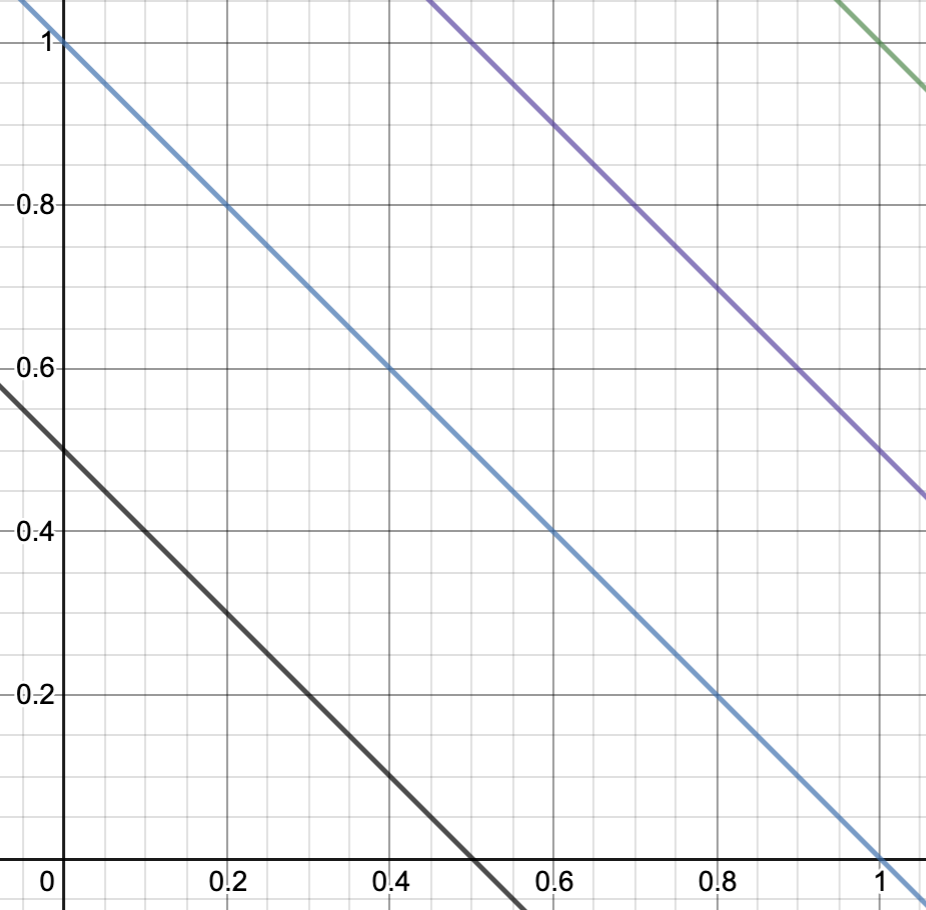
\includegraphics[scale=0.4]{linear_indiff}
\end{figure}
To see an increasing function in two variables that is not quasiconcave, consider $u(x_1, x_2) = x_1^2 + x_2^2$. The indifference curve is in figure 2 on the next page.
Formulaically, the indiffernece curve is given by $x_2 = \sqrt{c - x_1^2}$.
\begin{figure}
\caption{ Non-quasiconcave preferences}
\centering
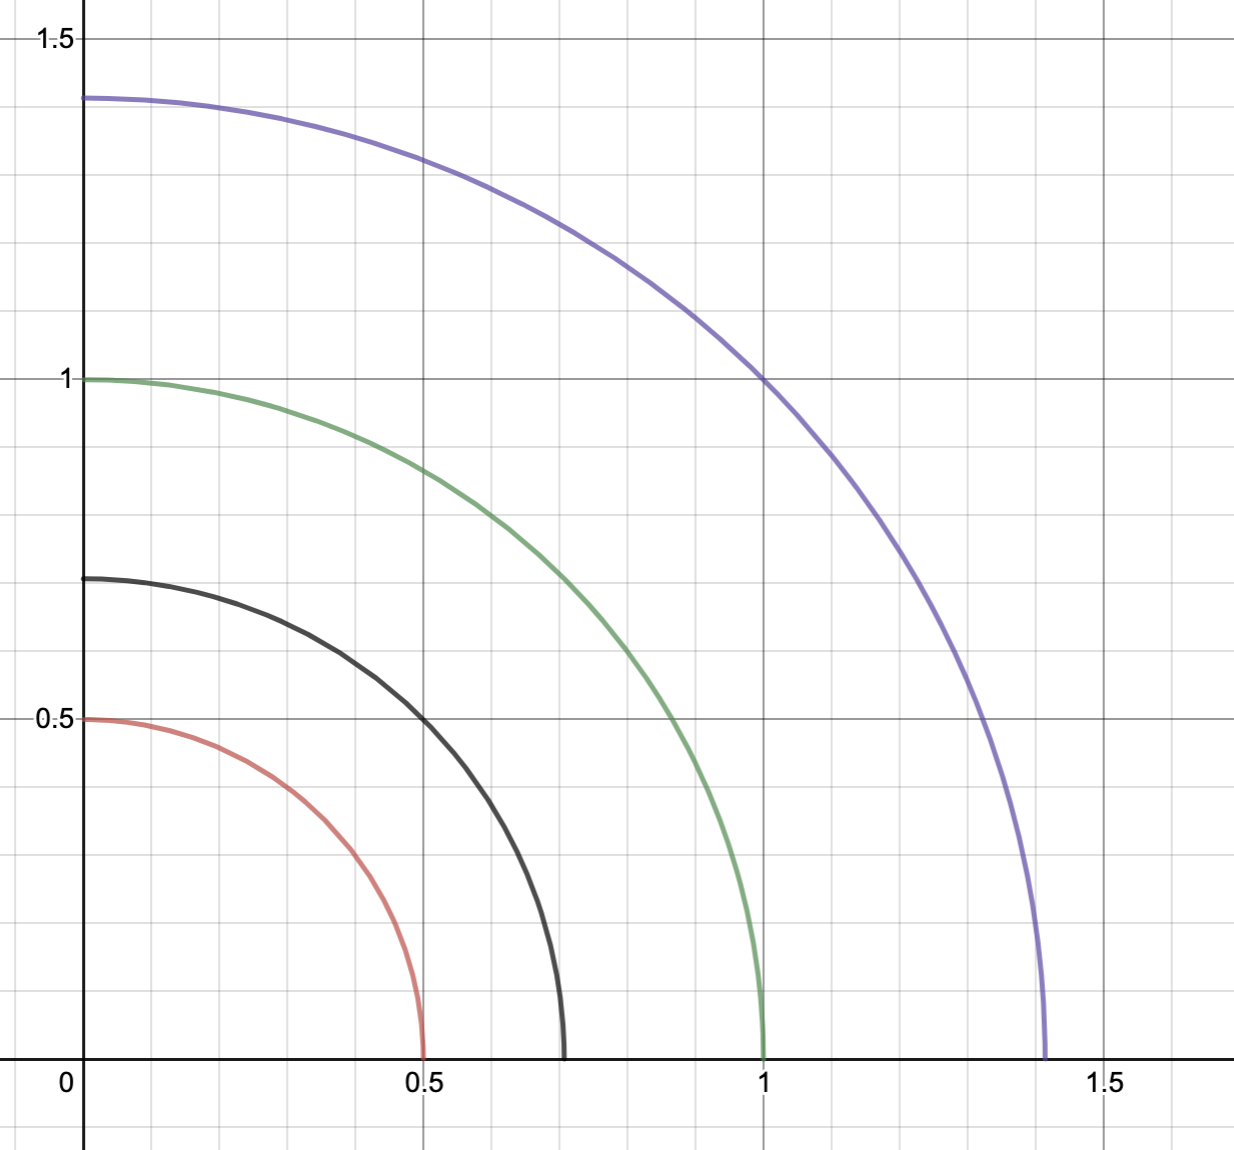
\includegraphics[scale=0.4]{concave_indiff}
\end{figure}
\paragraph{(2.2)}
The FOCs are solved for a point where the gradient of the budget constraint is a scalar multiple (by the factor of the Lagrange multiplier) of the gradient of the indifference curve, else pick a boundary point of the budget constraint. For our examples given previously, we note that FOCs will yield a maximizer for the first case in Figure 1 (linear case, so the FOC solution will typically be a boundary point, unless the prices are equal, in which case the entire budget constraint is a solution). However, in the second case shown in Figure 2, the FOC solution is actuallly interior in the budget constraint: however, a maximizer should be a boundary point for these indifference curves, and hence the FOCs fail to provide a maximizer.
\paragraph{(2.3)}
The indifference curve is given by $u(x_1, x_2) = c$. The slope of the indifference curve can be given by
\[ - \frac{\partial u / \partial x_1}{ \partial u / \partial x_2} \]
For sake of convenience, define
\[ \frac{\partial u}{\partial x_i} = u_i \]
\[ \frac{\partial^2 u}{\partial x_i \partial x_j} = u_{ij} \]
Lastly, let $dx_2/dx_1$ denote the slope of the indifference curve we found above. Differentiating the $dx_2/dx_1$ with respect to $x_1$, we get
\[ - \frac{u_2 \left(u_{11} + u_{12} (dx_2/dx_1) \right) - u_1 \left( u_{21} + u_{22}(dx_2/dx_1) \right) }{u_2^2} \]
\[ =- \frac{u_2 \left(u_{11} - (u_1/u_2) u_{12}\right) - u_1 \left( u_{21} - (u_1/u_2)u_{22} \right) }{u_2^2} \]
\[=-\frac{\left(u_2^2u_{11} - u_1 u_2 u_{12}\right) - \left( u_1 u_2 u_{21} - u_1^2 u_{22} \right) }{u_2^3}\]
\[=\frac{2u_1u_2u_{12} - u_2^2u_{11} - u_1^2 u_{22} }{u_2^3}\]
Note that the sign of this expression is the sign of the second derivative of the indifference curve. If the sign of this is positive (or if the RHS is 0), we have quasiconcavity. This implies
\[ 2 u_1 u_2 u_{12} \ge u_2^2 u_{11} + u_1^2 u_{22} \]
is a sufficient condition for quasiconcavity.

We now prove a lemma for the sake of a sanity check, and because we will need it later. Specifically, we claim that our condition for indifference curve convexity is invariant under an increasing monotone transformation $f$ on $u$.

Denote $f' = \partial f/\partial u$ and $f'' = \partial^2 f/\partial u^2$. We have that, by the chain rule
\[ (f \circ u)_1 = u_1 f' \]
\[ (f \circ u)_2 = u_2 f' \]
\[ (f \circ u)_{11} = u_1^2 f'' + u_{11} f'\]
\[ (f \circ u)_{22} = u_2^2 f'' + u_{22} f'\]
\[ (f \circ u)_{12} = u_{12} f' + u_1 u_2 f''\]
Then we note that
\[ 2(f \circ u)_1(f \circ u)_2(f \circ u)_{12} - (f \circ u)_2^2(f \circ u)_{11} - (f \circ u)_1^2(f \circ u)_{22} \]
\[ = 2(f')^2u_1u_2(u_{12} f' + u_1 u_2 f'') - u_2^2 (f')^2(u_1^2 f'' + u_{11} f') - u_1^2(f')^2(u_2^2 f'' + u_{22} f') \]
\[ = (f')^2 \left( 2u_1u_2(u_{12} f' + u_1 u_2 f'') - u_2^2(u_1^2 f'' + u_{11} f') - u_1^2(u_2^2 f'' + u_{22} f') \right) \]
\[ = (f')^2 \left( 2u_1u_2u_{12} f' + 2u_1^2 u_2^2 f'' - u_2^2u_1^2 f'' - u_2^2 u_{11} f' - u_1^2u_2^2 f'' - u_1^2 u_{22} f' \right) \]
\[ = (f')^2 \left( 2u_1u_2u_{12} f'  - u_2^2 u_{11} f' - u_1^2 u_{22} f' \right) \]
\[ = (f')^3 \left( 2u_1u_2u_{12}  - u_2^2 u_{11} - u_1^2 u_{22} \right) \]
Since $f' > 0$ ($f$ is by assumption monotonically increasing), we have that our condition for the convexity of indifference curves is invariant under application of $f$ to $u$, and hence we have shown our lemma.
\paragraph{(2.4)}
We now argue that diminishing marginal utility is neither sufficient nor necessary for indifference curve convexity. Let us examine the condition for indifference curve convexity:
\[ 2u_1 u_2 u_{12} \ge u_1^2 u_{22} + u_2^2 u_{11} \]
Now, we note that if $u_{12} >> 0$, it is possible for $u_{22}$ and $u_{11}$ to be both positive while satisfying this condition (i.e. consider $u = x_1^2y_1^2$). On the other hand, if $u_{12} << 0$ then it is possible to have both $u_{22}$ and $u_{11}$ be negative but still fail the condition.

Examine the condition we found:
\[ 2u_1u_2u_{12} \ge u_1^2 u_{22} + u_2^2 u_{11}\]

We note that if $u_{12} = 0$, and $u_1(0) = 0$ and $u_2(0) = 0$ then we must have both
\[ u_{22} \le 0\]
\[ u_{11} \le 0\]
We note that if $u_{12} = 0$, it is obvious that diminshing marginal utility implies that our condition holds. Now, we show that diminishing marginal utility is necessary for the condition if $u_1(0) = 0$ and $u_2(0) = 0$.
To show this, we use contradiction. Suppose $u_{11} > 0$ (logic is symmetric for $u_{22} > 0$). Then since $u_{12} = 0$, we have
\[ - u_1^2 u_{22} \ge u_2^2 u_{11} \]
\[ u_{22} \le - \frac{u_2^2}{u_1^2}u_{11} \]
Then, integrating with respect to $x_1$ over both sides from $a$ to $1$ and noting $u_2$ has no dependence on $x_1$ (since $u_{12} = 0$), we get
\[ \int_a^1 u_{22} dx_1 \le - \int_a^x \frac{u_2^2}{u_1^2}u_{11} dx_1 \]
\[ u_{22} (1-a) \le \frac{u_2^2}{u_1(1)} - \frac{u_2^2}{u_1(a)} \]
But taking the limit as $a \to 0$, the RHS goes to $-\infty$ and the LHS goes to $u_{22}$, and hence this inequality is impossible. Therefore, this implies that our conditions imply that diminishing marginal utility is necessary for indifference curve convexity.

We note that a special case of our condition occurs for utilities of the form
\[ u(x_1, x_2) = g(x) + h(y)\]
where
\[ g'(0) = 0 \]
\[ h'(0) = 0 \]
We also note that by the lemma we proved in the previous part, any monotonically increasing transformation $f$ on such a utility preserves the condition; as a special case, we note that the CES utilities are a monotonically increasing transform $f(t) = t^{1/\rho}$ on such a utility ($g(t) = h(t) = t^\rho$) and hence for CES utilities, diminishing marginal utility is an equivalent condition to indifference curve convexity.

The underlying principle for convexity of the indifference curves is diminishing marginal rate of substitution, not diminishing marginal utility. We have noted that for a large class of utility functions (including many of the common utilites economists work with), the conditions on diminishing marginal rate of substitution are equivalent by diminishing marginal utility. Hence, maybe it is a little overzealous for Millicent to sue.
\paragraph{(2.5)}
\begin{itemize}
\item[--] Take a C-D utility:
\[ u = x_1^\alpha x_2^{\beta} \]
The FOCs are
\[ \alpha x_1^{\alpha-1} x_2^{\beta} = \lambda p_1 \]
\[ \beta x_1^{\alpha} x_2^{\beta - 1} = \lambda p_2 \]

The demand functions are:
\[ x_1(p,w) = \frac{\alpha w}{p_1(\alpha + \beta)} \]
\[ x_2(p,w) = \frac{\beta w}{p_2(\alpha + \beta)} \]
The indirect utility function is then
\[ v(p,w) = w^{\alpha + \beta}\frac{\alpha^\alpha\beta^\beta }{p_1^\alpha p_2^{\beta} (\alpha + \beta)^{\alpha + \beta}}\]
Then
\[ \frac{\partial v(p,w)}{\partial w} = w^{\alpha + \beta - 1}\frac{\alpha^\alpha\beta^\beta }{p_1^\alpha p_2^{\beta}(\alpha + \beta)^{\alpha + \beta - 1}} \]
Note the Lagrange multiplier is
\[\frac{\alpha}{p_1} \left(\frac{\alpha w}{p_1(\alpha + \beta)}\right)^{\alpha-1}\left( \frac{\beta w}{p_2(\alpha + \beta)} \right)^{\beta}  \]
\[ = w^{\alpha + \beta - 1}\frac{\alpha^\alpha\beta^\beta }{p_1^\alpha p_2^{\beta} (\alpha + \beta)^{\alpha + \beta - 1}}  \]
As desired.
\item[--]
If $u$ represents $\succeq$, then $x \succeq y$ iff $u(x) \ge u(y)$. But if $f$ is a strictly increasing transformation, then $u(x) \ge u(y)$ iff $f(u(x)) \ge f(u(y))$. Hence $x \succeq y$ iff $f(u(x)) \ge f(u(y))$, and hence $f \circ u$ represents $\succeq$.
\item[--]
As computed in the first part, the marginal utility of income is
\[ w^{\alpha + \beta - 1}\frac{\alpha^\alpha\beta^\beta }{p_1^\alpha p_2^{\beta} (\alpha + \beta)^{\alpha + \beta - 1}} \]
If we take the transformation $f_c(t) = t^{\frac{c}{\alpha + \beta}}$, and take the new utility $f_c \circ u$, then the only things that have changed are the Cobb-Douglas parameters:
\[ \alpha' = \frac{\alpha c}{\alpha + \beta} \]
\[ \beta' = \frac{\beta c}{\alpha + \beta} \]
and the marginal utility of income is
\[ w^{\alpha' + \beta' - 1}\frac{\alpha'^{\alpha'}\beta'^{\beta'} }{p_1^{\alpha'} p_2^{\beta'} (\alpha' + \beta')^{\alpha' + \beta' - 1}}  = w^{c-1} \frac{\alpha'^{\alpha'}\beta'^{\beta'} }{p_1^{\alpha'} p_2^{\beta'} (c-1)^{c-1}}\]
Note if we take the transformation $f_1$, we have no $w$ dependence. If we take the transformation $f_2$, we have the marginal utility of income is increasing in $w$. If we take the transformation $f_{1/2}$, the marginal utility of income is decreasing in income.
\item[--] The utilities for individuals 1 and 2 are:
\[ v_1(p,w) = w^{\alpha_1 + \beta_1}\frac{\alpha_1^{\alpha_1}\beta_1^{\beta_1} }{p_1^{\alpha_1} p_2^{\beta_1} (\alpha_1 + \beta_1)^{\alpha_1 + \beta_1}} \]
\[ v_2(p,w) = w^{\alpha_2 + \beta_2}\frac{\alpha_2^{\alpha_2}\beta_2^{\beta_2} }{p_1^{\alpha_2} p_2^{\beta_2} (\alpha_2 + \beta_2)^{\alpha_2 + \beta_2}} \]
Clearly, by using the transformation $f_1(t)= t + v_2(p,w)$ on $u_1$, we can ensure that 1 has a higher utility, when comparing $f_1 \circ u_1$ and $u_2$. Similarly, the tranformation $f_2(t) = t + v_1(p,w)$ ensures that when comparing $u_1$ and $f_2 \circ u_2$, individual 2 has a higher utility. In terms of marginal utility:
\[ \lambda_1  = w^{\alpha_1 + \beta_1 - 1}\frac{\alpha_1^{\alpha_1}\beta_1^{\beta_1} }{p_1^{\alpha_1} p_2^{\beta_1} (\alpha_1 + \beta_1)^{\alpha_1 + \beta_1 - 1}} \]
\[ \lambda_2  = w^{\alpha_2 + \beta_2 - 1}\frac{\alpha_2^{\alpha_2}\beta_2^{\beta_2} }{p_1^{\alpha_2} p_2^{\beta_2} (\alpha_2 + \beta_2)^{\alpha_2 + \beta_2 - 1}}\]
Taking the transformation $f_1(t) = k t^{1/(\alpha_1 + \beta_1)}$, the marginal utility of income becomes
\[ \lambda'_1  = k \frac{\alpha_1^{\alpha_1}\beta_1^{\beta_1} }{p_1^{\alpha_1} p_2^{\beta_1}} \]
Taking the transformat $f_2(t) = j t^{1/(\alpha_2 + \beta_2)}$, the marginal utility of income for individual 2 becomes
\[ \lambda'_2  = j \frac{\alpha_2^{\alpha_2}\beta_2^{\beta_2} }{p_1^{\alpha_2} p_2^{\beta_2}} \]
We then see that since $\alpha, \beta > 0$, $p_1, p_2 \ge 0$, we can pick $k, j$ to make either $\lambda'_1$ or $\lambda'_2$ greater, however we wish.
\item[--] There isn't really a grounds for progressive taxation on utility maximization theory alone; however, the grounds can be made on a subjective grounds by examining the marginal decrease in consumption in a wealthier consumption compared to the marginal increase in consumption for a poorer person, and making a value judgment on whether the consumption tradeoff is worthwhile (i.e., if a rich person loses a sport car with a unit less of wealth, but a poorer person with the unit would consume more basic necessities, we might make a subjective call that this is a worthwhile tradeoff). The site is misleading; whether Millicent should sue is up to her value judgment on the cost of suing versus her perceived benefit.
\end{itemize}


\end{document}
	% line of code telling latex that your document is ending. If you leave this out, you'll get an error
